\documentclass[tikz,border=0pt]{standalone}
\usepackage[american]{circuitikz}
\usetikzlibrary{arrows.meta,calc,positioning,decorations.pathmorphing,patterns}
\definecolor{zyloTeal}{HTML}{174A5B}
\definecolor{zyloTealTwo}{HTML}{246B7A}
\definecolor{zyloInk}{HTML}{1F2933}
\definecolor{zyloSoft}{HTML}{EAF4F4}
\definecolor{zyloPaper}{HTML}{F8FAFB}
\definecolor{zyloLine}{HTML}{44606B}
\definecolor{zyloOrange}{HTML}{D97706}
\begin{document}
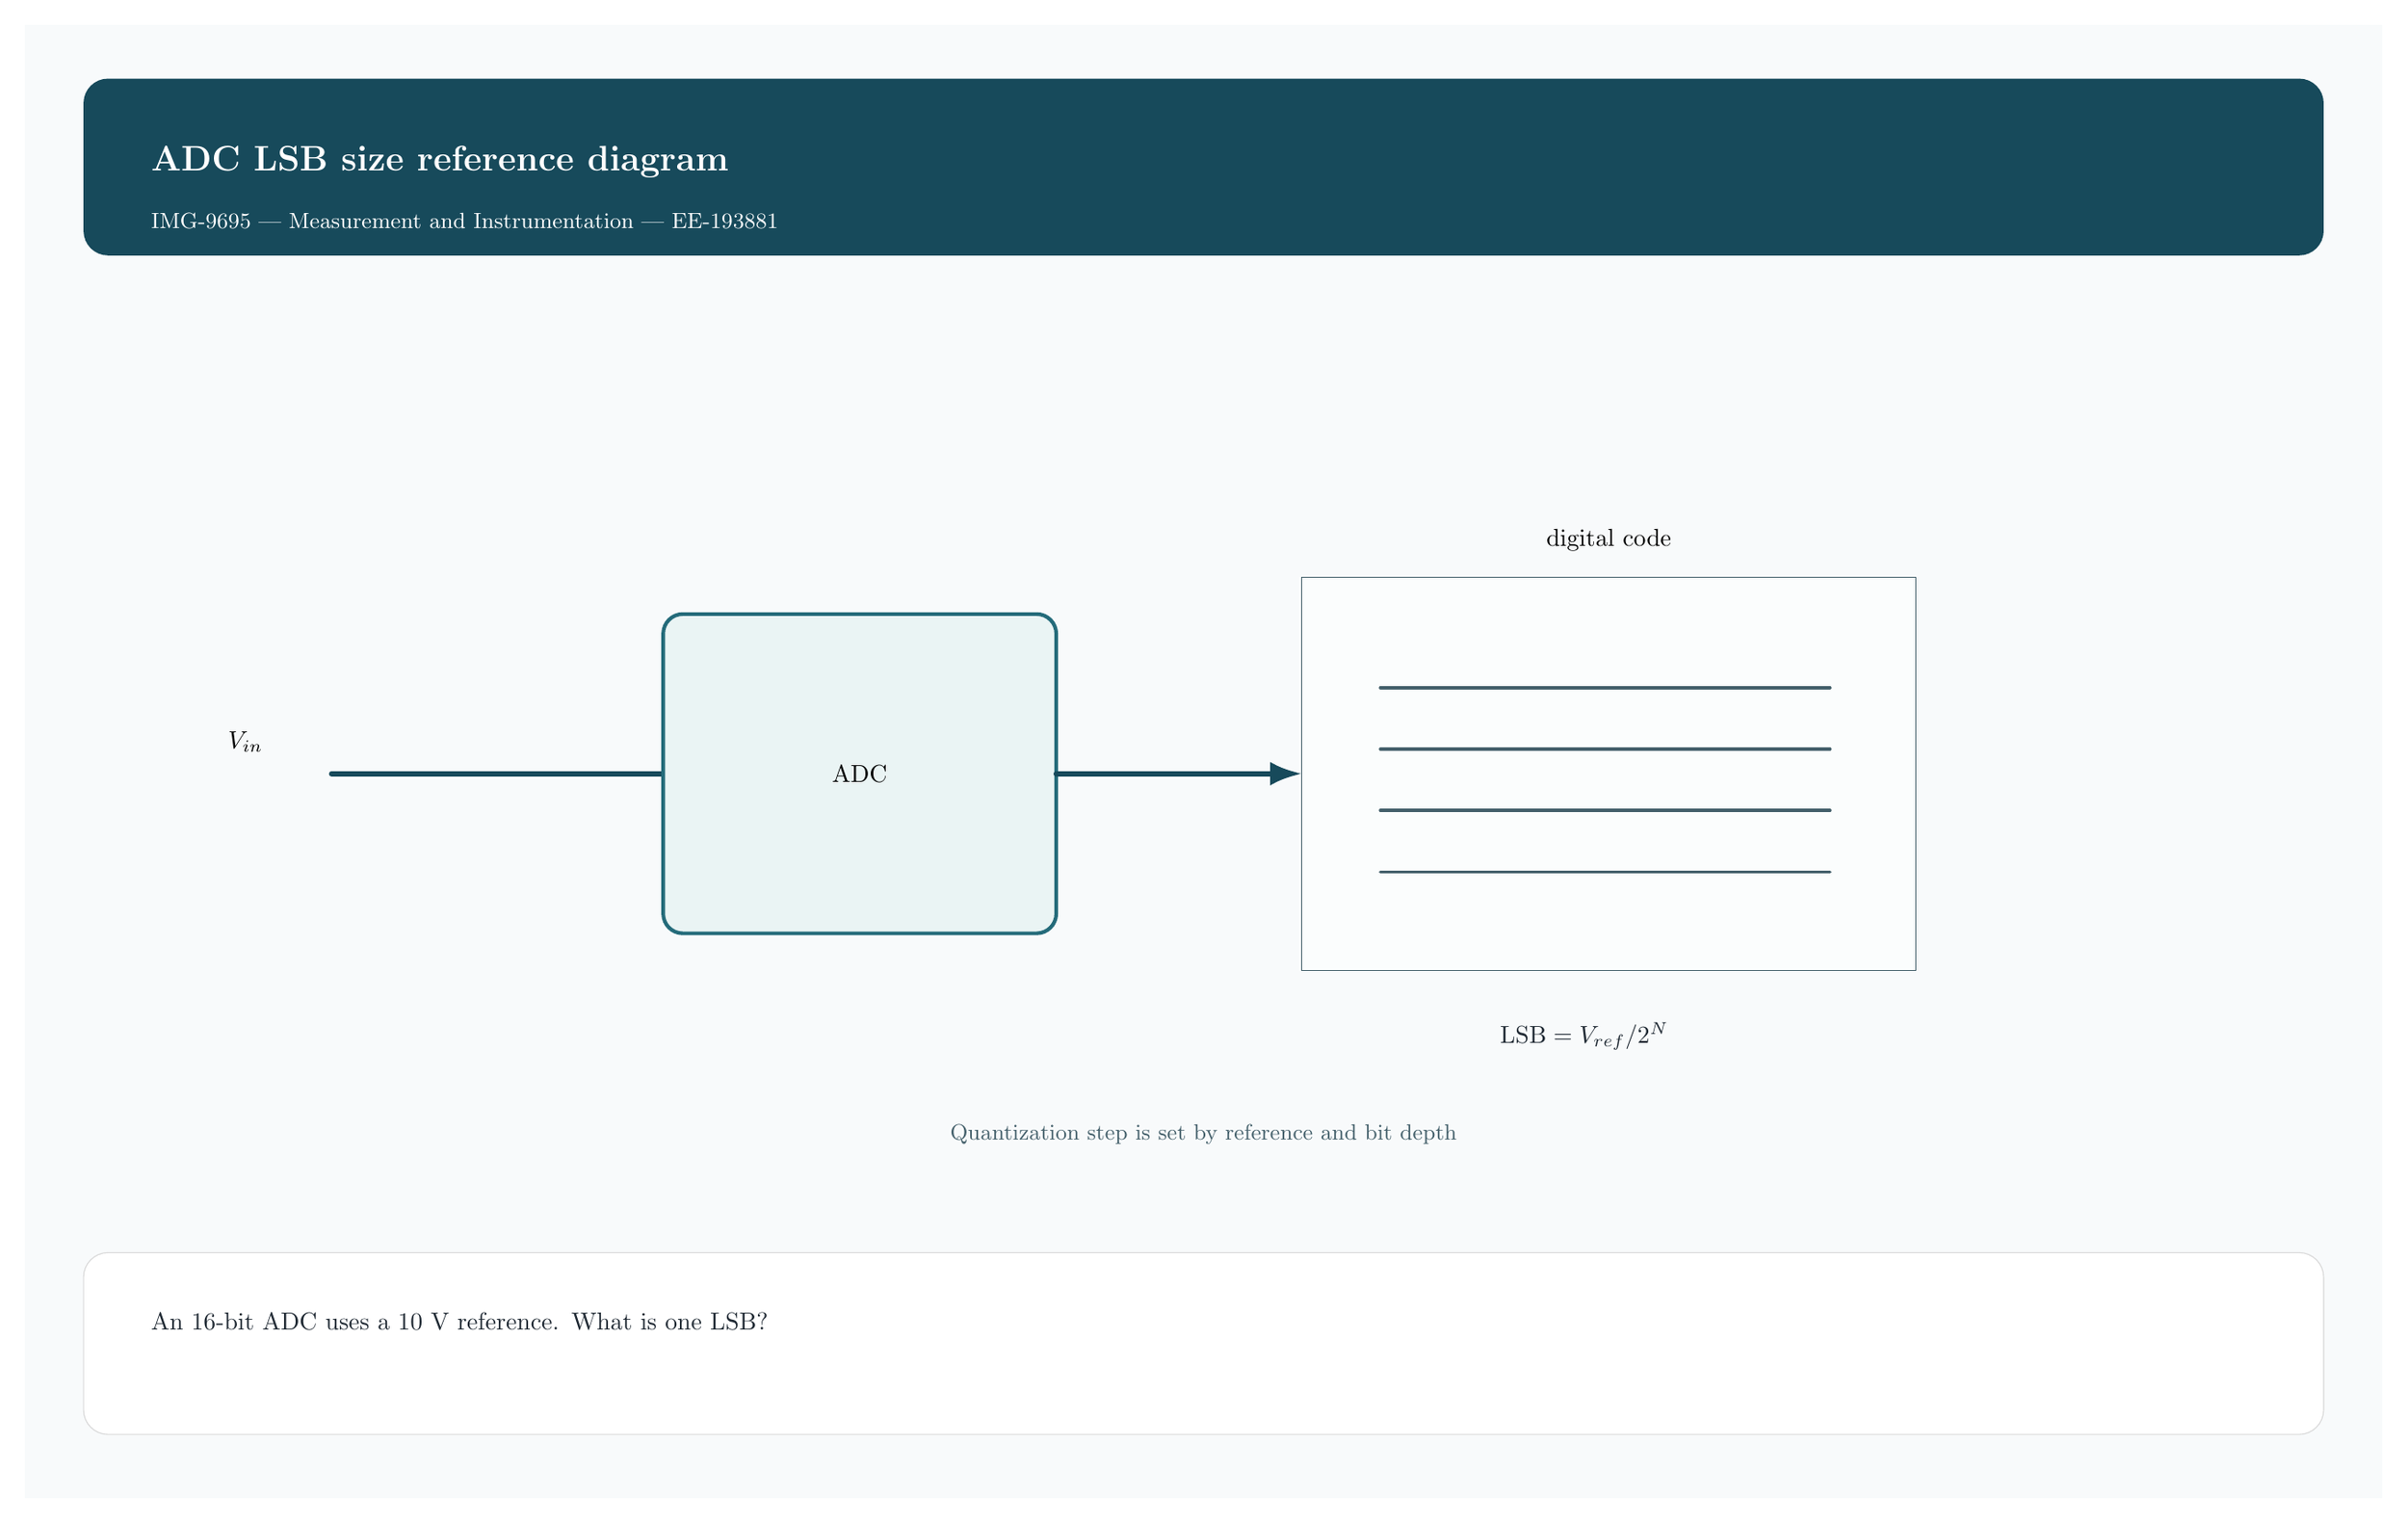
\begin{tikzpicture}[x=1pt,y=-1pt,>=Latex,line cap=round,line join=round]
\path[fill=zyloPaper] (0,0) rectangle (960,600);
\path[fill=zyloTeal,rounded corners=10pt] (24,22) rectangle (936,94);
\node[anchor=west,text=white,font=\bfseries\Large] at (48,56) {ADC LSB size reference diagram};
\node[anchor=west,text=white!82,font=\small] at (48,80) {IMG-9695 | Measurement and Instrumentation | EE-193881};
\tikzset{wire/.style={draw=zyloTeal,line width=2.2pt},thinwire/.style={draw=zyloLine,line width=1.35pt},accent/.style={draw=zyloOrange,line width=2.2pt},box/.style={draw=zyloTealTwo,fill=zyloSoft,line width=1.5pt,rounded corners=8pt}}
\draw[wire] (125,305) -- (260,305);
\node[box,minimum width=160pt,minimum height=130pt] at (340,305) {ADC};
\draw[wire,->] (420,305) -- (520,305);
\node[draw=zyloLine,fill=white!80!zyloSoft,minimum width=250pt,minimum height=160pt] at (645,305) {};
\node at (645,210) {digital code}; \draw[thinwire] (552,270) -- (735,270); \draw[thinwire] (552,295) -- (735,295); \draw[thinwire] (552,320) -- (735,320); \draw[thinwire] (552,345) -- (735,345);
\node[text=zyloInk] at (635,412) {$\mathrm{LSB}=V_{ref}/2^N$}; \node at (90,292) {$V_{in}$};
\node[font=\small,text=zyloLine] at (480,452) {Quantization step is set by reference and bit depth};
\path[draw=black!15,fill=white,rounded corners=10pt] (24,500) rectangle (936,574);
\node[anchor=west,text width=860pt,align=left,text=zyloInk,font=\normalsize] at (48,528) {An 16-bit ADC uses a 10 V reference. What is one LSB?};
\end{tikzpicture}
\end{document}
